\documentclass{lab}

\renewcommand{\AA}{\ensuremath{\mathring{A}}}

\begin{document}

\labtitle{4.3.1}{Изучение дифракции света}{2~мая~2019~г.}{16~мая~2019~г.}

\section*{Постановка эксперимента}

\begin{quote}
	\textbf{{\normalsize Цель работы: }}
	исследовать явления дифракции Френеля и Фраунгофера на щели, изучить влияние дифракции на разрешающую способность оптических инструментов.
\end{quote}

\begin{quote}
	\textbf{{\normalsize Оборудование: }}
	оптическая скамья, ртутная лампа, монохроматор, щели с регулируемой шириной, рамка с вертикальной нитью, двойная щель, микроскоп на поперечных салазках с микрометрическим винтом, зрительная труба.
\end{quote}

\section*{Выполнение работы}

\subsection*{Дифракция Френеля на щели}

\begin{figure}[H]
	\centering
	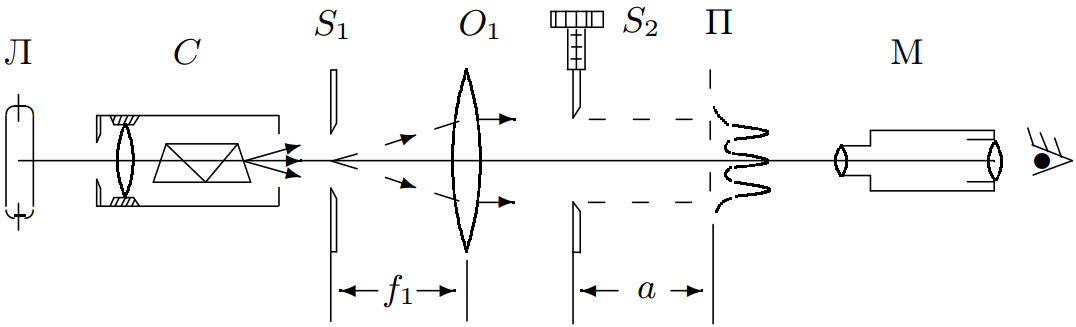
\includegraphics[width = \textwidth]{scheme-1}
	\caption{Схема установки для наблюдения дифракции Френеля на щели}
	\label{scheme-1}
\end{figure}

Проведем настройку установки согласно приведенному в лаборатории описанию работы. Также некоторые характеристики: $ f_1 = 12.5~см, f_2 = 16~см $.\\

Ширина щели, измеренная с помощью ее собственного микрометрического винта:
\begin{equation}
D \approx 200~мкм
\end{equation}

Снимем зависимость координаты микроскопа и количества темных полос на дифракционной картине. Результаты представим в таблице \ref{tab-1}.
\begin{table}[H]
	\centering
	\begin{tabular}{|c|cccc|}
		\hline
		$ n $ & 1 & 2 & 3 & 4 \\
		$ a,~см $ & 57.2 & 56.8 & 56.6 & 56.5 \\ \hline
	\end{tabular}
	\caption{Зависимость координаты микроскопа и количества темных полос на дифракционной картине}
	\label{tab-1}
\end{table}

Ширина щели $ S_2 $ совпадает с ранее полученным результатом и равна $ 200~мкм $.\\

По результатам измерений таблицы \ref{tab-1} получим зависимость полуширины щели от количества зон Френеля.
\begin{equation}
m = n + 1, ~~~~~ 2\xi_m = 2\sqrt{am\lambda}, ~~~~~ где ~ \lambda = 5461 \AA
\end{equation}

\newpage

Теперь запишем зависимость полуширины щели от количества зон Френеля.
\begin{table}[H]
	\centering
	\begin{tabular}{|c|cccc|}
		\hline
		$ m $ & 2 & 3 & 4 & 5 \\
		$ 2\xi_m,~мкм $ & 213 & 260 & 300 & 335 \\ \hline
	\end{tabular}
	\caption{Зависимость полуширины щели от количества зон Френеля}
	\label{tab-2}
\end{table}

По данным таблицы \ref{tab-2} построим график зависимости полуширины щели от количества зон Френеля.
\begin{figure}[H]
	\centering
	\begin{tikzpicture}
	
	\pgfplotstableread{
		X	Y		x-err	y-err
		2	213		00		5
		3	260		00		5 
		4	300		00		5
		5	335		00		5
	}{\mytable}
	
	\begin{axis}[
	width = 0.8\textwidth,
	grid = major,
	xlabel = $ m $,
	ylabel = $ 2\xi_m \text{, мкм} $,
	xmin = 1.5,
	ymin = 200,
	xmax = 5.5,
	ymax = 360
	]
	
	\addplot[
	only marks,
	color = red,
	mark = *,
	error bars/.cd,
	x dir = both,
	x explicit,
	y dir = both,
	y explicit
	]
	table[
	x error = x-err,
	y error = y-err
	] {\mytable};
	
	\addplot[
	mark = none,
	color = red
	]
	table[
	y = {create col/linear regression={y=Y}}
	] % compute a linear regression from the
	{\mytable};
	
	\end{axis}
	\end{tikzpicture}
	\caption{Зависимость полуширины щели от количества зон Френеля}
	\label{g_1}
\end{figure}

Что касается распределения света и тени при дифракции на краю экрана, при увеличении расстояния от края экрана осцилляция интенсивности уменьшается, а с само значение $ I $ стремится к $ I_0 $.

Также не перемещая микроскоп, но изменяя ширину щели, можно пронаблюдать следующие явления:

\begin{enumerate}
	\item при увеличении ширины щели дифракционная картина уменьшается, боковые полосы съезжаются к нулевому максимуму.
	
	\item при уменьшении ширины щели, наоборот, дифракционная картина увеличивается и боковые полосы разъезжаются от нулевого максимума.
\end{enumerate}

Также можно пронаблюдать дифракцию Френеля на препятствии, поставив вместо щели $ S_2 $ рамку с тонкой вертикальной нитью.

При этом можно убедиться, что картина на нити ведет себя подобным образом, за исключением направления максимума. Из-за него всегда можно наблюдать светлый центр и четное число темных полос.

\subsection*{Дифракция Фраунгофера на щели}

\begin{figure}[H]
	\centering
	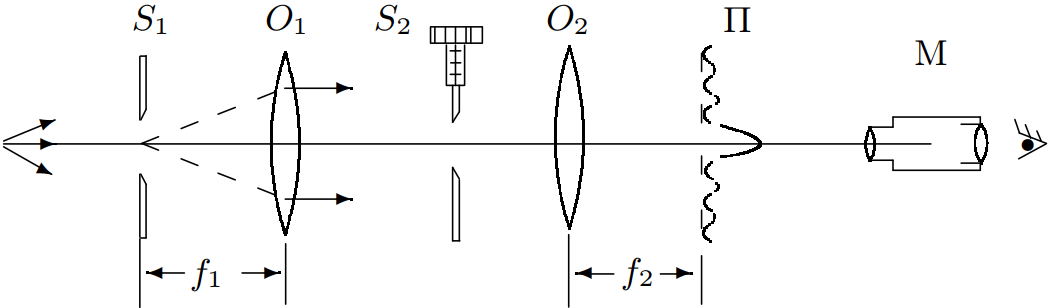
\includegraphics[width = \textwidth]{scheme-2}
	\caption{Схема установки для наблюдения дифракции Фраунгофера на щели}
	\label{scheme-2}
\end{figure}

С помощью поперечного винта микроскопа снимем зависимость координаты $ x_m $ от номера минимума.
\begin{table}[H]
	\centering
	\begin{tabular}{|c|cccccccccc|}
		\hline
		$ m $ & -5 & -4 & -3 & -2 & -1 & 0 & 1 & 2 & 3 & 4 \\
		$ x_m,~дел $ & 16 & 33 & 55 & 75 & 95 & 115 & 136 & 155 & 174 & 199 \\ \hline
	\end{tabular}
	\caption{Зависимость координаты $ x_m $ от номера минимума}
	\label{tab-3}
\end{table}

Построим график по таблице \ref{tab-3}.
\begin{figure}[H]
	\centering
	\begin{tikzpicture}
	
	\pgfplotstableread{
		X	Y		x-err	y-err
		-5	16		00		5
		-4	33		00		5 
		-3	55		00		5
		-2	75		00		5
		-1	95		00		5
		0	115		00		5
		1	136		00		5
		2	155		00		5
		3	174		00		5
		4	199		00		5
	}{\mytable}
	
	\begin{axis}[
	width = 0.8\textwidth,
	grid = major,
	xlabel = $ m $,
	ylabel = $ x_m \text{, дел} $,
	ymin = 0,
	ymax = 220
	]
	
	\addplot[
	only marks,
	color = red,
	mark = *,
	error bars/.cd,
	x dir = both,
	x explicit,
	y dir = both,
	y explicit
	]
	table[
	x error = x-err,
	y error = y-err
	] {\mytable};
	
	\addplot[
	mark = none,
	color = red
	]
	table[
	y = {create col/linear regression={y=Y}}
	] % compute a linear regression from the
	{\mytable};
	
	\end{axis}
	\end{tikzpicture}
	\caption{Зависимость координаты $ x_m $ от номера минимума}
	\label{g_2}
\end{figure}

По наклону графика (рис. \ref{g_2}) находим: $ \Delta x = 20.2~дел $.
\begin{equation}
D = \dfrac{f_2 \lambda}{\Delta x} = 216~мкм, \text{что близко к измеренному ранее значению ширины щели.}
\end{equation}

Также можно убедиться в том, что смещение щели $ S_2 $ в боковом напрвлении не приводит к сдвигу дифракционной картины.

Это можно объяснить тем фактом, что изображение всегда улавливается в фокальной плоскости линзы, в то время как лучи распараллеливаются линзой $ O_2 $ вне зависимости от перемещения $ S_2 $.\\

Также лишний раз убеждаемся, что дифракционная картина Фраунгофера меняется согласно формуле $ \Delta x = f_2 \lambda / D $ или $ x_m = f_2 m \lambda / D $.

Это означает, что полосы разъезжаются и становятся шире при уменьшении $ D $.

\subsection*{Дифракция Фраунгофера на двух щелях}

\begin{figure}[H]
	\centering
	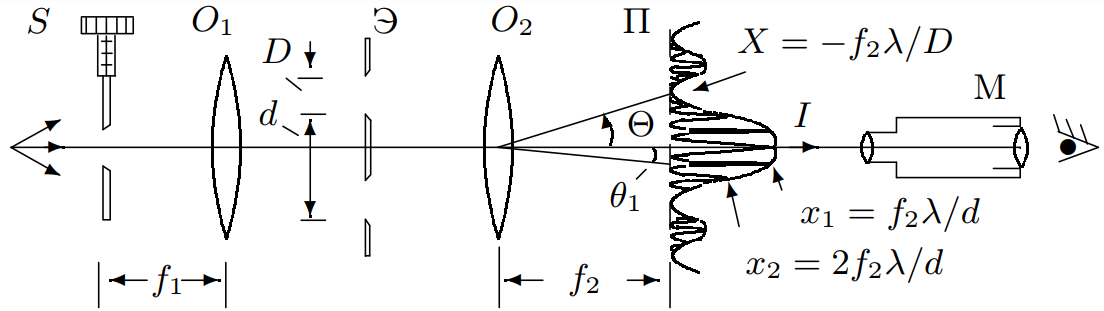
\includegraphics[width = \textwidth]{scheme-3}
	\caption{Схема установки для наблюдения дифракции Фраунгофера на двух щелях}
	\label{scheme-3}
\end{figure}

Определим с помощью поперечного винта микроскопа расстояние между самыми удаленными друг от друга темными полосами и посчитаем число светлых полос между ними: $ \delta x = 35~мкм, ~ N = 17~полос $.

Ширина центрального максимума примерно $ 0.6~мм $.
\begin{equation}
d = \dfrac{f_2 \lambda}{\delta x} = 0.86~мм, \text{что совпадает с измеренным значением} ~ d = 0.84~мм.
\end{equation}
\begin{equation}
b = \dfrac{f_1 \lambda}{d} = 0.05~мм, \text{что также совпадает с ранее установленным фактом.}
\end{equation}

Также было сделано наблюдение о влиянии интерференции от протяженного источника на дифракционную картину Фраунгофера.

Картина исчезает при $ b_0 = 0.1~мм $, однако затем восстанавливается с меньшей контрастностью.

\subsection*{Влияние дифракции на разрешающую способность оптического инструмента}

\begin{figure}[H]
	\centering
	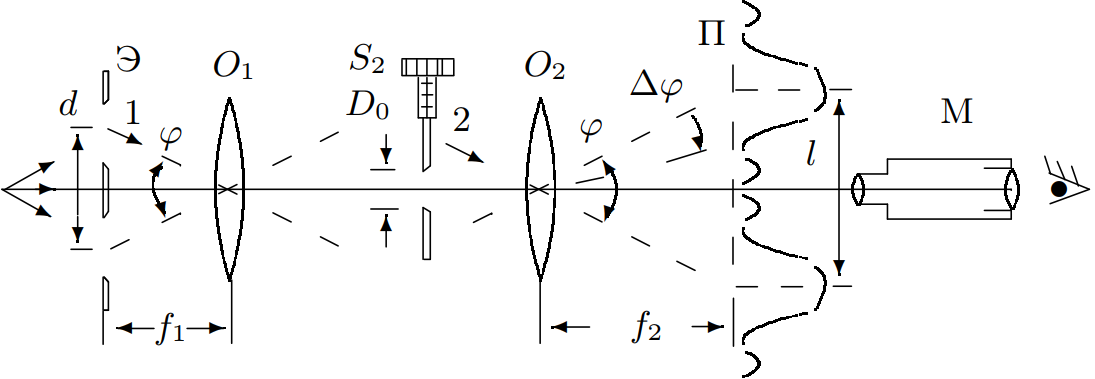
\includegraphics[width = \textwidth]{scheme-4}
	\caption{Схема установки для исследования разрешающей способности оптического инструмента}
	\label{scheme-4}
\end{figure}

Найдем изображение, которое не различает два различных источника и запишем ширину щели, соответствующую граничному случаю критерия Релея.
\begin{equation}
D_0 = 110 \cdot 0.001 = 0.11~мм = 110~мкм.
\end{equation}

Измерим координаты ширину каждой щели: $ h_1 = 0.13~мм, h_2 = 0.31~мм $. Расстояние между ними: $ d = 0.84~мм. $
\begin{equation}
D_0 = \dfrac{f_1 \lambda}{d} = 104~мкм, \text{что давольно точно совпадает с ранее полученным результатом.}
\end{equation}

\subsection*{Итоги}

Были исследованы дифракции Френеля и Фраунгофера на щели, влияние дифракции на разрешающую способность оптических инструментов.
Также была исследована дифракция Френеля на двух щелях и пронаблюдалось влияние интерференции от протяженного источника на видность основной картинки.

\end{document}